\begin{figure}
\centering
\captionsetup{justification=centering}

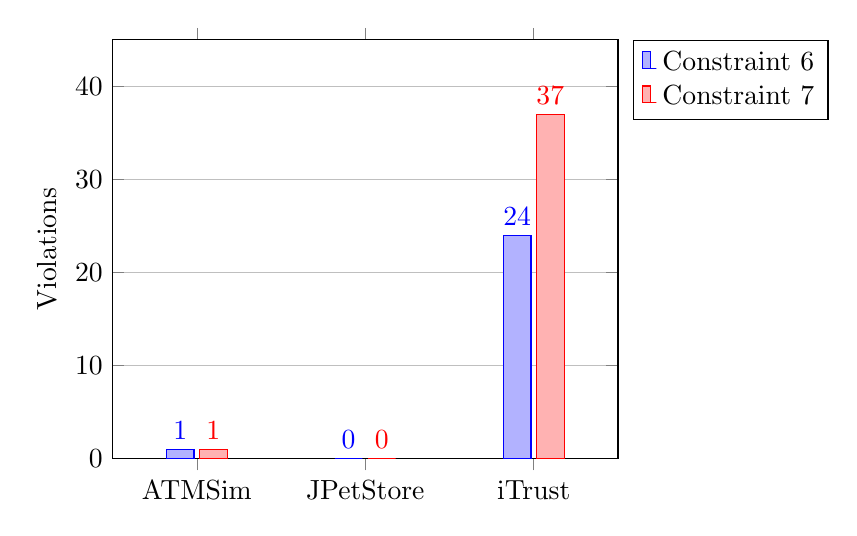
\begin{tikzpicture}
\begin{axis}[
    width=8cm,
    ybar,
    ymin = 0,
    ymax = 45,
    ymajorgrids = true,
    enlarge x limits=0.25,
    xbar legend,
    legend pos=outer north east,
    ylabel={Violations},
    symbolic x coords={ATMSim,JPetStore,iTrust},
    %xlabel={System},
    xtick=data,
    nodes near coords,
    nodes near coords align={vertical},
    ]
%C6
\addplot coordinates {(ATMSim,1) (JPetStore,0) (iTrust,24)};
%C7
\addplot coordinates {(ATMSim,1) (JPetStore,0) (iTrust,37)};

\legend{Constraint 6,Constraint 7}
\end{axis}
\end{tikzpicture}

\caption
    [Violations of constraint 6 and 7 found in iTrust when asserting ground truth]
    {The violations of constraint 6 and 7 found in iTrust when asserting ground truth.}
\label{bar:frequency_violation_extension}
\end{figure}